

\section{Koordinatensysteme mit Funktionaldeterminante}

\subsection{Polarkoordinaten}
\begin{figure}[h!]
\centering
    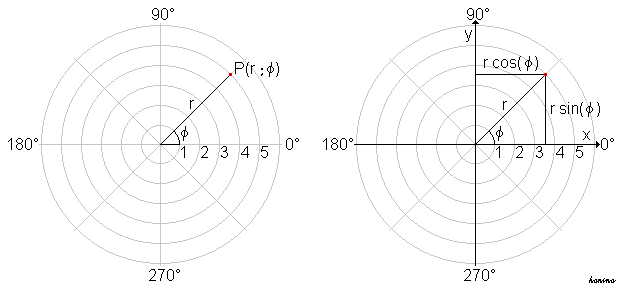
\includegraphics[width=0.6\textwidth]{images/Ebene_polarkoordinaten.PNG}
    \caption{Quelle: https://de.wikipedia.org/}
    
\end{figure}

Umrechnung erfolgt durch: \\
$x=r\cos\varphi$\\
$y=r\sin\varphi$\\

Aus den Umrechnungsformeln von Polarkoordinaten in kartesische Koordinaten erhält man für die Funktionaldeterminante als Determinante der Jacobi-Matrix:\\
\\$
\det J = \det\frac{\partial(x,y)}{\partial(r,\varphi)}
=\begin{vmatrix}
  \frac{\partial x}{\partial r} & \frac{\partial x}{\partial \varphi} \\
  \frac{\partial y}{\partial r} & \frac{\partial y}{\partial \varphi}
\end{vmatrix}
=\begin{vmatrix}
  \cos\varphi & -r\sin\varphi \\
  \sin\varphi &  r\cos\varphi
\end{vmatrix} =r\cos^2\varphi + r\sin^2\varphi = r
$

\subsection{Zylinderkoordinaten}
\begin{figure}[h!]
\centering
    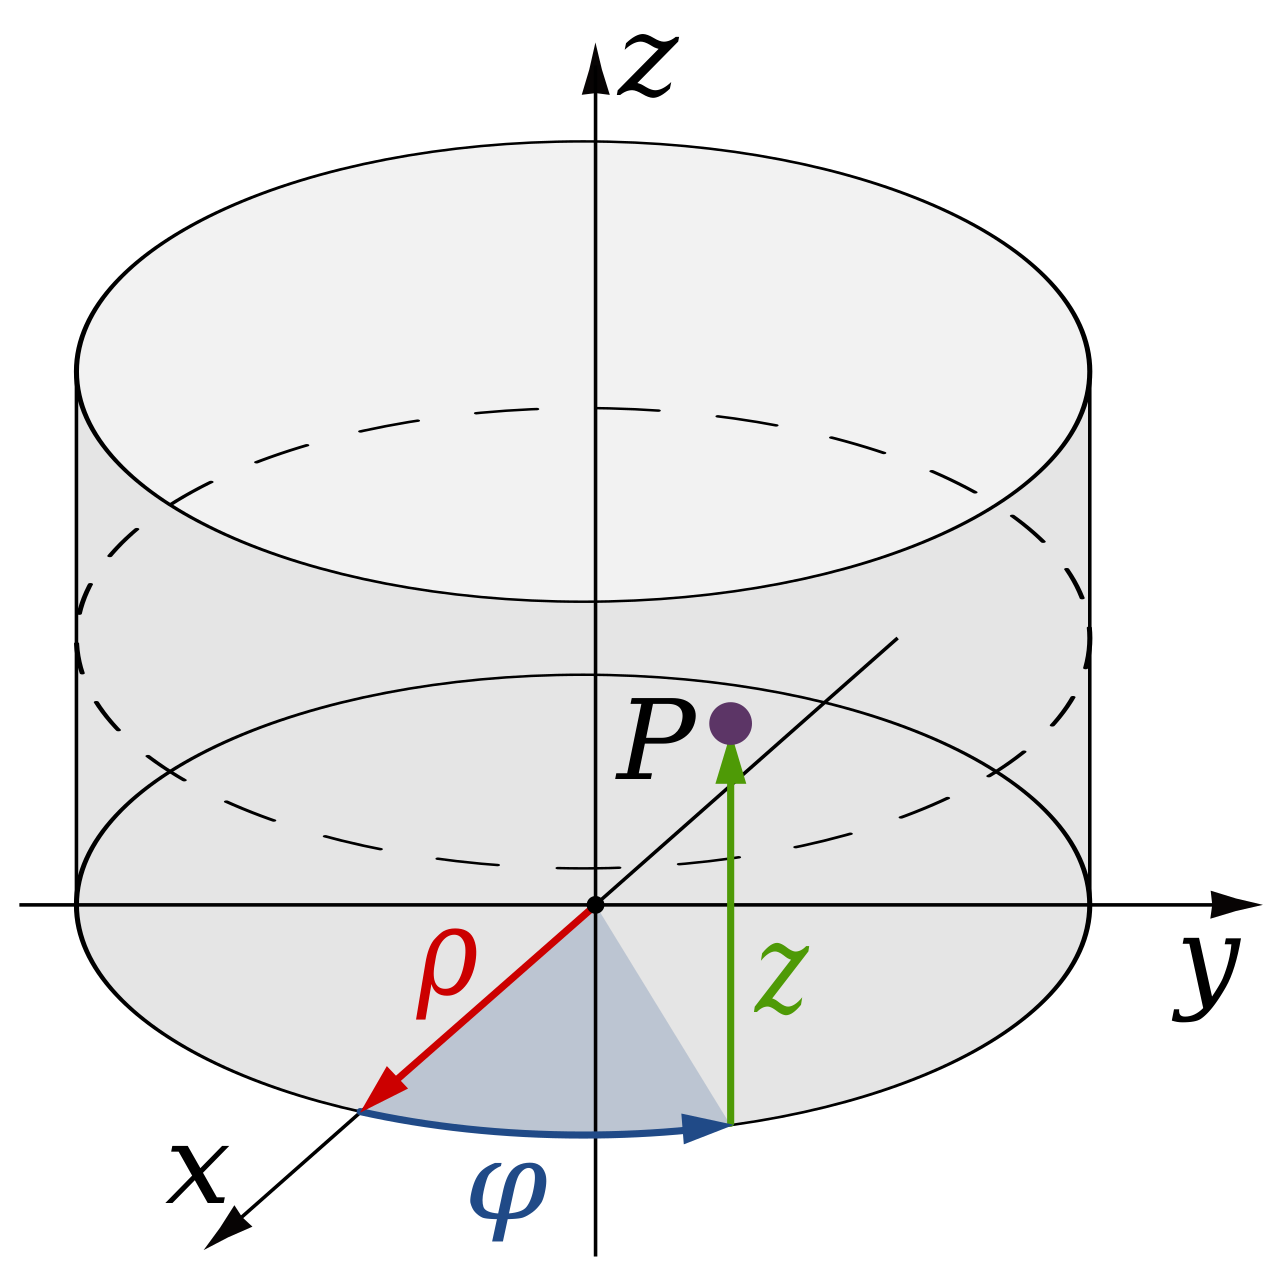
\includegraphics[width=0.3\textwidth]{images/zylinderkoord.png}
    \caption{Quelle: https://de.wikipedia.org/}
    
\end{figure}
Umrechnung erfolgt durch: \\
$x=\rho\ \cos\varphi$\\
$y=\rho\ \sin\varphi$\\
$z=z$\\

Mit Funktionaldeterminante:
$
\det\frac{\partial(x,y,z)}{\partial(\rho,\varphi,z)}=\begin{vmatrix}
  \cos\varphi & -\rho\sin\varphi & 0 \\
  \sin\varphi &  \rho\cos\varphi & 0 \\
            0 &                0 & 1
\end{vmatrix}=\rho$


\subsection{Kugelkoordinaten}
\begin{figure}[h!]
\centering
    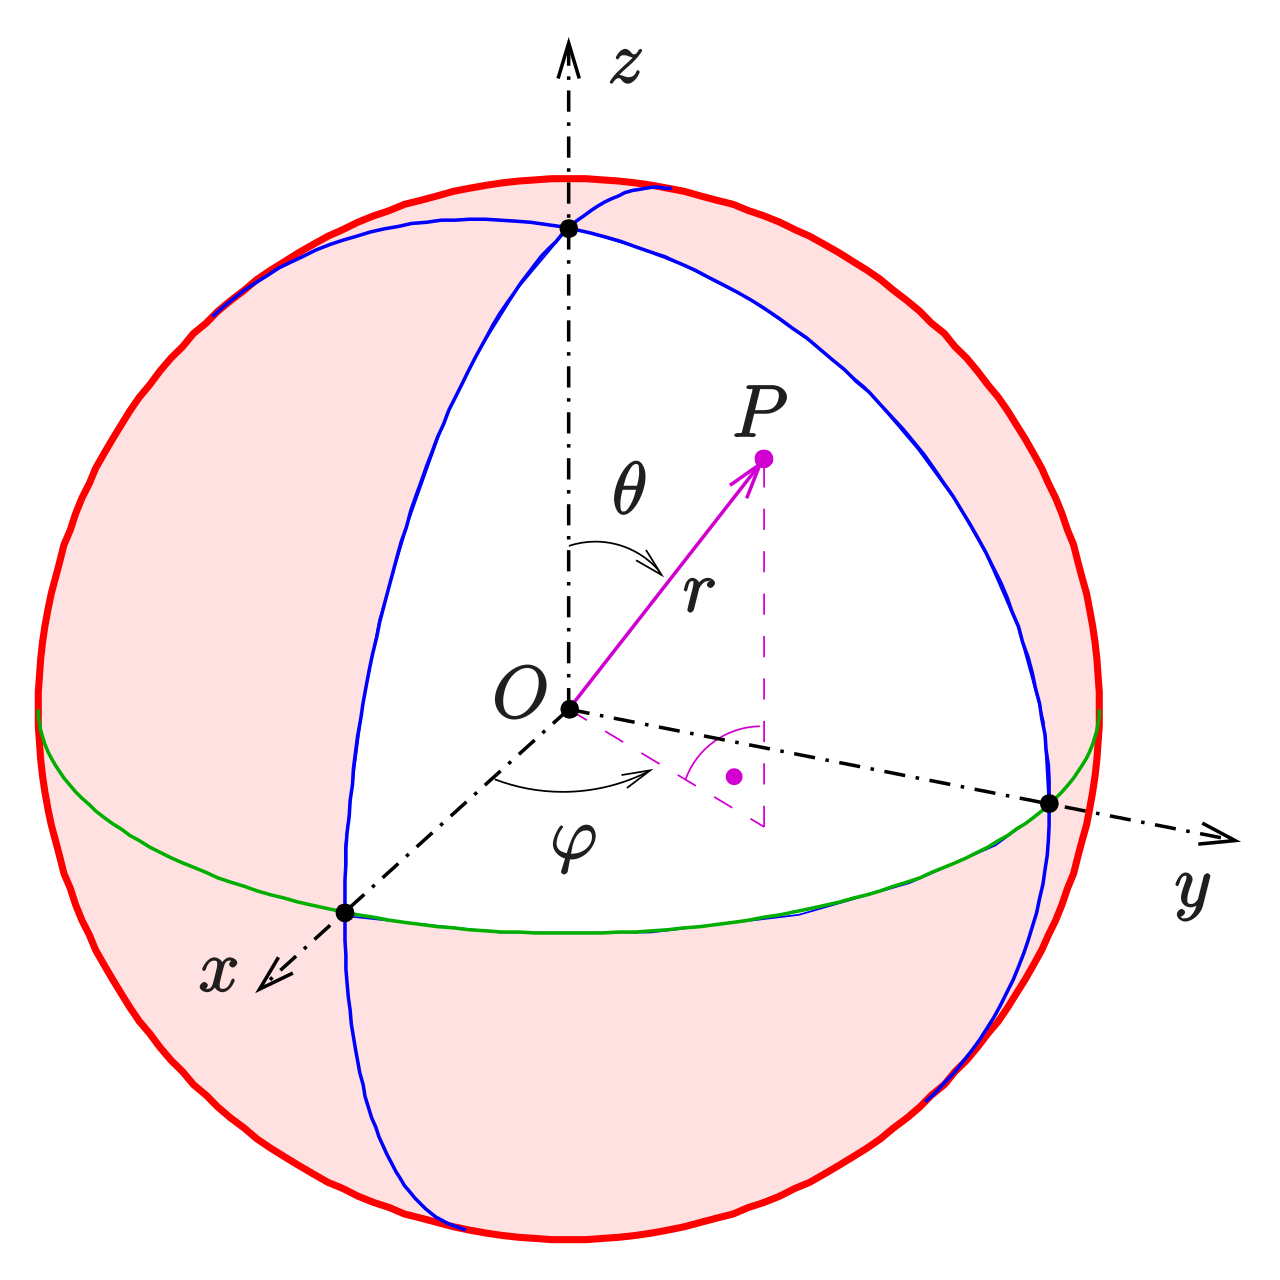
\includegraphics[width=0.4\textwidth]{images/kugelkoord.png}
    \caption{Quelle: https://de.wikipedia.org/}
    
\end{figure}

Umrechnung erfolgt durch: \\
$x = r \cdot \sin \theta \cdot \cos \varphi$ \\
$y = r \cdot \sin \theta \cdot \sin \varphi$ \\
$z = r \cdot \cos \theta$ \\

Jacobi-Matrix:

$J =\frac{\partial(x,y,z)}{\partial(r,\theta,\varphi)}
  =\begin{pmatrix}
     \sin\theta\cos\varphi&r\cos\theta\cos\varphi&-r\sin\theta\sin\varphi\\
     \sin\theta \sin\varphi&r\cos\theta\sin\varphi&r\sin\theta\cos\varphi\\
     \cos\theta&-r\sin\theta&0
   \end{pmatrix}$\\
   
   mit Funktionaldeterminante:
   $\det J=r^2\sin\theta$








\section{Rotationsmatrix, Drehmatrix}

\subsection{Drehmatrix der Ebene}
Jede Rotation um den Ursprung ist eine lineare Abbildung. Wie bei jeder linearen Abbildung genügt daher zur Festlegung der Gesamtabbildung die Festlegung der Bilder der Elemente einer beliebigen Basis. Wird die Standardbasis gewählt, sind die Bilder der Basisvektoren gerade die Spalten der dazugehörigen Abbildungsmatrix.

Wir haben unter $R_{\alpha}$ \\
\\
 $\begin{pmatrix} 1 \\ 0 \end{pmatrix} \mapsto \begin{pmatrix} \cos\alpha \\ \sin\alpha \end{pmatrix}
\qquad\text{und}\qquad
\begin{pmatrix} 0 \\ 1 \end{pmatrix} \mapsto \begin{pmatrix} -\sin\alpha \\ \cos\alpha \end{pmatrix}$ \newline

Die Drehmatrix für eine Drehung um $\alpha$ ist also:  \newline
$R_\alpha = \begin{pmatrix} \cos\alpha & -\sin\alpha \\ \sin\alpha & \newline \cos\alpha\end{pmatrix}$

 $\begin{pmatrix} x' \\ y' \end{pmatrix} = \begin{pmatrix} \cos\alpha & -\sin\alpha \\ \sin\alpha & \cos\alpha\end{pmatrix} \cdot \begin{pmatrix} x \\y \end{pmatrix}$\\

\subsubsection{Herleitung}
\begin{figure}[H] 
\centering
    {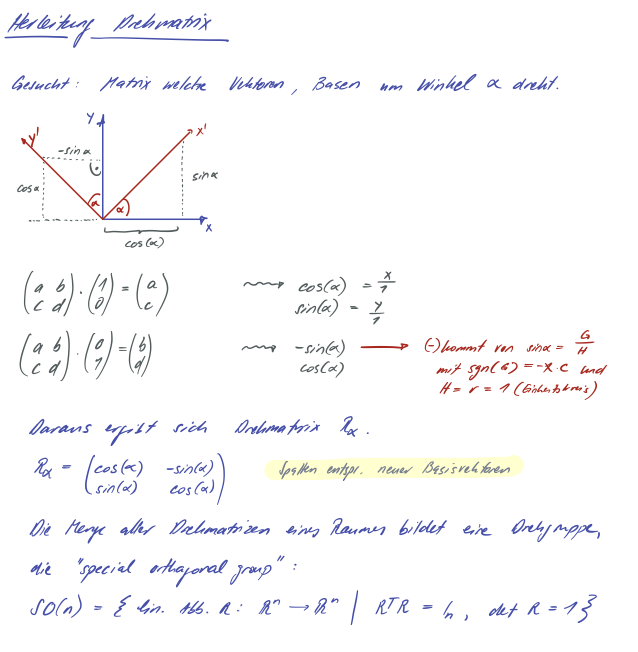
\includegraphics[width=0.75\textwidth]{images/herldrehmat.png}}
    \caption{Quelle: Miles Strässle, 20.11.2019}    
\end{figure}

\subsection{Drehmatrix in 3-Dimensionen}
In der Physik werden häufig Drehungen des Koordinatensystems benutzt, dann müssen bei den untenstehenden Matrizen die Vorzeichen aller Sinus-Einträge vertauscht werden. Die Drehung eines Vektors um einen bestimmten Winkel in einem Koordinatensystem ist äquivalent zur Drehung des Koordinatensystems um den gleichen Winkel in umgekehrter Richtung (Drehung um negativen Winkel). 
\vspace{0.5cm}
„Der Drehsinn ergibt sich, wenn man entgegen der positiven Drehachse auf den Ursprung sieht.“

\subsubsection{Drehung um die x-Achse:}
$R_x(\alpha) = \begin{pmatrix}
1 &   0         & 0           \\
0 & \cos \alpha & -\sin \alpha \\
0 & \sin \alpha &  \cos \alpha
\end{pmatrix}$
\subsubsection{Drehung um die y-Achse:}
$R_y(\alpha) = \begin{pmatrix}
\cos \alpha  & 0 & \sin \alpha \\
   0         & 1 &  0          \\
-\sin \alpha & 0 & \cos \alpha
\end{pmatrix}$
\subsubsection{Drehung um die z-Achse:}
$R_z(\alpha) = \begin{pmatrix}
\cos \alpha & -\sin \alpha & 0 \\
\sin \alpha &  \cos \alpha & 0 \\
   0        &  0           & 1
\end{pmatrix}$


